\chapter{绪论}\label{chap:introduction}

\section{研究背景}
随着信息技术的快速发展,人工智能、物联网等技术与智能终端的结合得越来越紧密,在智能终端上除了为用户提供基础服务以外还要提供更智能化的服务。因此,智能终端上要承担的计算任务越来越重。但目前智能终端上所拥有的计算、存储等资源并没有跟上对于智能终端计算能力的需求。与此同时,家庭、办公楼等智能终端环境中还存在着很多相对空闲、计算资源没有得到充分利用的计算设备。越来越重的计算任务与计算资源分配不均的矛盾日益凸显,为了解决这样的矛盾,在整体资源有限的情况下使资源利用达到最优化,我们想到可以使用多个智能终端协同提供服务,提供一种能够整合多终端资源、合理利用多终端资源的服务技术。
\section{研究意义}
本研究针对智能终端计算任务越来越重与终端计算资源分布不均衡的问题,引入容器技术,对于多终端上的资源进行聚合管理,并通过多智能终端协同技术,合理分配利用终端空闲资源,提高智能终端的服务效率以及智能终端的资源利用率,为未来智能终端为用户提供日常生活服务以及与边缘计算、人工智能、物联网等技术的结合打下良好基础,具有重要的研究意义和应用价值。
\section{研究内容}
为了解决终端计算能力跟不上以及终端空闲资源浪费的问题,引入多终端协同服务。引入后会面对如何使用多终端上的空闲资源、提高利用率、管理等问题。
引入了多终端协同技术和容器技术以后,整个系统会存在很多单一终端服务不会遇到的问题,本研究中主要解决其中的四个问题,包括基于容器化多终端服务系统架构设计、基于容器化服务资源提供技术、资源受限终端任务调度策略、基于预测的容器弹性服务策略。

本文针对上面提出的几个问题,首先介绍了边缘计算技术、容器虚拟化技术、计算迁移技术、任务调度算法、预测算法等相关技术和算法的研究现状,分析其目前还存在的问题。本文结合容器虚拟化技术和多终端协同服务技术,设计了基于容器化的多终端协同服务系统,并主要研究系统中的基于容器的多终端透明计算迁移技术、多终端协同服务任务调度算法优化以及基于预测的终端弹性服务技术。

本文具体研究内容如下:
\begin{enumerate}
    \item 随着计算机技术的快速发展和边缘计算技术的逐渐成熟,位于网络边缘的用户终端设备在用户的数字化生活中正扮演着越来越重要的角色,其定位逐渐从单一的用户服务发起者向用户服务的提供者转变。这会使用户终端承担越来越多的计算任务,这也对终端设备的服务质量和计算能力提出了越来越高的要求。但另一方面,边缘终端设备上还存在着大量没有得到充分利用的空闲资源。终端对计算能力要求越来越高与终端设备资源利用率不高之间存在着可以提升的空间,使用多终端协同服务技术来提升终端整体可用计算能力、提升终端整体资源利用率称为一种可行的方法。但是多终端协同服务技术还是会存着不少问题,如:终端资源管理、终端服务管理、多终端节点管理、节点组网等问题。为了解决这些问题,本文设计了基于容器化的多终端协同服务系统,引入容器虚拟化技术对多终端资源进行虚拟化,形成资源池,可以为上层终端服务按需使用;还参考微服务架构,提出多终端协同服务系统架构,可以进行终端服务管理;另外还提出了去中心化的自组织网络结构,进行多终端节点管理和节点组网。
    \item 相比云端协同计算,边缘终端设备距离用户更近,而且拥有很多空余资源没有得到充分利用,如何将这部分距离用户更近、成本更低的资源组织利用起来为用户设备提供计算迁移服务也成为了多终端协同服务技术中的一个值得研究的问题。为了将多终端上空闲的资源整合利用起来,为终端用户提供服务,提升用户体验,我们以HTML5中的Web Worker方法为例,研究Web应用透明计算迁移到以容器形式部署在边缘设备上的服务端,设计并实现了一种基于容器的Web Worker透明边缘计算迁移方法。一系列实验结果证明,所提出的方法能够将用户终端周围设备的空闲资源利用起来,为用户提供计算迁移服务,减少计算总执行时间,提高终端整体资源利用率,有效提高用户体验。
    \item 为了在终端资源有限且终端资源异构性极强的情况下,合理调度任务请求到更合适的执行节点上,使得任务总体开销更小,减少响应时间,提高用户体验,本研究基于一种群体智能的演进式优化算法————蝗虫优化算法,提出一种带有随机跳出机制的动态权重蝗虫优化算法来解决优化问题。在该算法中,我们在原有蝗虫优化算法的基础上,增加了基于完全随机跳出因素的跳出机制,来提高算法的跳出局部最优的能力。另外,我们还根据搜索阶段的不同,使用动态的权重参数来代替原算法中的线性递减搜索单元权重参数,帮助算法在不同的搜索阶段获得更大的迭代收益。经过一系列测试函数的实验验证,我们提出的带有随机跳出机制的动态权重蝗虫优化算法能够有效提高优化算法的搜索精度及收敛速度。在此基础上,我们进一步提出一种改进蝗虫优化算法,并将其应用于解决多终端任务调度问题。在该算法中,我们引入变型的sigmoid函数作为非线性舒适区调节参数,增强算法的搜索能力。同时,我们提出基于Levy飞行的局部搜索机制,让搜索单元在局部拥有一定的“搜索视觉”,提高算法的局部搜索能力。另外,我们还使用基于线性递减参数的随机跳出策略,增强算法跳出局部最优能力,并将成功跳出的结果影响力维持若干次迭代。经过一系列测试函数和标准测试集的实验,实验结果表明我们提出的改进蝗虫优化算法能够有效提高优化算法的搜索精度、稳定性、搜索到更优解的可能性及收敛速度。最后我们提出了终端上任务调度问题的数学模型,并将提出的改进蝗虫优化算法应用到该问题的求解过程中。实验结果证明,我们提出的改进蝗虫算法在求解终端上任务调度问题时能够得到很好的效果。
    \item 对于终端服务系统来说,如果不进行终端服务预部署,则当用户服务请求到达终端服务系统的时候现场启动基于Docker容器的终端服务端程序还是会消耗一定时间,尽管相比于传统的VM虚拟机,Docker容器技术的启动时间已经非常短了,但这个启动时间相比于用户请求等待响应时间仍然较长,不能接受。但是如果提前进行终端服务预部署,虽然可以达到缩短用户请求等待响应时间的目的,但是对于资源有限的终端来说,等待用户服务请求到达的过程会消耗大量额外的资源,同样是不能接受的。这就形成了一个矛盾的问题。为了解决是否进行预部署的问题,本研究提出了一种基于预测的容器弹性服务策略,利用改进的卡尔曼滤波算法,对未来一小段时间的用户请求流量进行预测,并根据预测结果对终端服务的容器规模进行适当调整,以达到在不增加用户请求响应等待时间、不降低用户体验的情况下对终端资源利用更合理的目的。经过一系列的仿真实验,证明所提出的基于预测的容器弹性服务策略能够有效根据用户请求流量的变化趋势动态调整终端服务规模,合理利用终端资源。
\end{enumerate}
\section{本文内容安排}
本文一共分为七个章节,针对基于容器化的多终端协同服务技术进行研究,组织结构如图\ref{fig:introduction_framework_of_organization}所示,各章节内容概述如下:
\begin{figure}[!htbp]
    \centering
    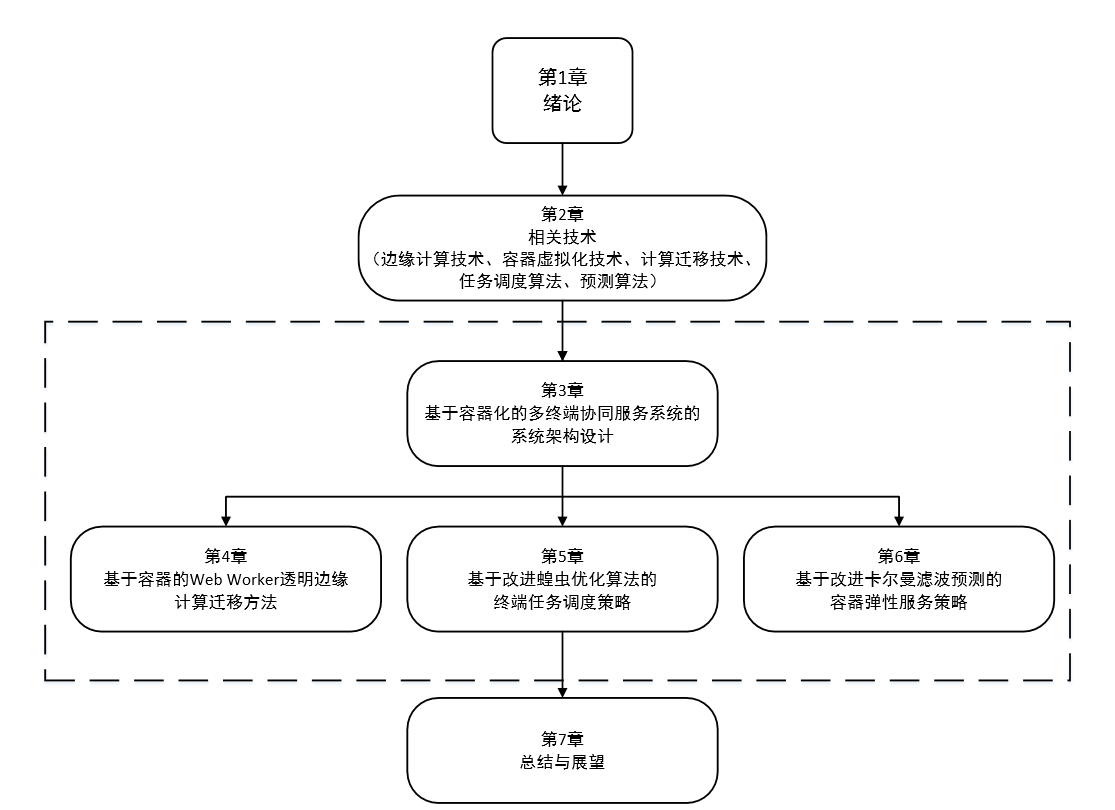
\includegraphics[width=1.0\textwidth]{Introduction_Framework_of_Organization_Temp}
    \caption{论文组织结构}
    \label{fig:introduction_framework_of_organization}
\end{figure}


第1章介绍了基于容器化的多终端协同服务技术的发展背景以及研究意义、本文的研究内容和本文内容安排。

第2章介绍了基于容器化的多终端协同服务技术的相关技术的研究现状,包括边缘计算技术、容器虚拟化技术、计算迁移技术、任务调度算法、预测算法等相关技术和算法。

第3章结合容器虚拟化技术和微服务架构,提出了基于容器化的多终端协同服务系统的系统架构设及构建方法,解决了多终端节点管理、终端资源管理、终端服务管理等问题。后面三个研究点均为本章提出的系统中的部分具体实现。

第4章提出了一种基于容器的Web Worker透明边缘计算迁移方法,以透明计算迁移的方式将终端空闲资源利用起来为用户终端提供服务,减少任务计算执行时间,提高用户体验。

第5章提出了一种带有随机跳出机制的动态权重蝗虫优化算法来解决优化问题。并在此基础上提出了一种改进蝗虫优化算法,更进一步地提高了算法的性能,解决了终端任务调度问题。

第6章结合卡尔曼滤波算法,提出了一种基于预测的容器弹性服务策略,解决终端服务是否进行预部署的问题。

第7章总结了上述研究工作,并对未来工作进行了展望。